\documentclass[10pt]{beamer}

\usepackage{appendixnumberbeamer}

% \usepackage{beamerposter}

\usepackage{fontspec}
\usepackage{csquotes}
\usepackage[main=english]{babel}
\babelprovide[import, onchar=ids fonts letters]{ancientgreek}

\newcommand{\Bernoulli}{\text{Bernoulli}}
\newcommand{\LogNormal}{\text{LogNormal}}
\newcommand{\Normal}{\text{Normal}}
\newcommand{\Dirichlet}{\text{Dirichlet}}
\newcommand{\Exponencial}{\text{Exponencial}}
\newcommand{\logit}{\text{logit}}
\newcommand{\Dist}{\text{Dist}}
\newcommand{\Cop}{\text{Cop}}
\newcommand{\Sent}{\text{Sent}}
\newcommand{\Auth}{\text{Auth}}
\newcommand{\PoS}{\text{PoS}}
\newcommand{\Th}{\text{Th}}
\newcommand{\Dia}{\text{Dia}}
\newcommand{\abar}{\overline{\alpha}}
\newcommand{\bbar}{\overline{\beta}}
\newcommand{\bv}[1]{\beta_\text{#1}}
\newcommand{\bvi}[1]{\beta_{\text{#1}_i}}

\usepackage{linguex}
\usepackage{tikz} %for all basic options
\usepackage{tikz-qtree} %for simple tree syntax
\usepackage{booktabs}
\usepackage[normalem]{ulem}
\usepackage{hyphenat}
\usepackage{multirow}
\usepackage{pgfplots}
\usepackage{paralist}
\usepackage[
  backend=biber,
  uniquename=init,
  giveninits,
  dashed=true,
  style=authoryear-comp
  ]{biblatex}
\addbibresource{./biblio.bib}

\usetheme[
	progressbar=foot,
	sectionpage=progressbar,
	numbering=fraction]{metropolis}

\newcommand\Wider[2][4em]{%
	\makebox[\linewidth][c]{%
		\begin{minipage}{\dimexpr\textwidth+#1\relax}
			\raggedright#2
		\end{minipage}%
	}%
}

\title{Repensando atração de caso em orações infinitivas do grego antigo}
\author{Caio B. A. Geraldes\newline<\texttt{caio.geraldes@usp.br}>\vspace{5pt}}
\date{1º de dezembro de 2025}
\institute{Universidade de São Paulo\\
\includegraphics[height=0.40cm]{logo-fapesp.png}}

\setsansfont{Fira Sans}
\setmonofont[Scale=0.75]{Noto Sans Mono}

\definecolor{obl}{RGB}{41,5,195}
\definecolor{teste}{RGB}{46,139,87}
\definecolor{verb}{RGB}{255, 0, 0}
\definecolor{acc}{RGB}{11,92,16}
\definecolor{atr}{RGB}{128,0,128}
\newcommand{\Vum}[1]{#1}
\newcommand{\Vdois}[1]{#1}
\newcommand{\Obl}[1]{\textcolor{obl}{\uline{#1}}}
\newcommand{\XAcu}[1]{\textcolor{acc}{\uline{#1}}}
\newcommand{\XObl}[1]{\textcolor{atr}{\uline{#1}}}
\newcommand{\vum}[1]{\textbf{#1}}
\newcommand{\vdois}[1]{\textbf{#1}}
\newcommand{\oobl}[1]{\textbf{#1}}
\newcommand{\xobl}[1]{\textbf{#1}}

\begin{document}

\maketitle

\begin{frame}
  \frametitle{Exemplo}

  \ex.
  \a.συμβουλεύει \textbf{τῷ Ξενοφῶντι ἐλθόντα} {εἰς Δελφοὺς}
  ἀνακοινῶσαι {τῷ θεῷ} {περὶ τῆς πορείας}.\\
  Ele aconselha Xenofonte ir a Delfos e interrogar o deus sobre a viagem.
  (Xen.\ \emph{Anab.} 3.1.5)
  \b.ἀφῆκε \textbf{μοι ἐλθόντι} {πρὸς ὑμᾶς} λέγειν τἀληθῆ.\\
  Ele permitiu a mim vir e falar frente a vós a verdade.
  (Xen.\ \emph{Hell.} 6.1.13)


\end{frame}

\begin{frame}
  \frametitle{Grafo direcionado acíclico: Concordância}
  Modelo teórico: \textcite{Corbett2006}

  Traços do \textbf{C}ontrolador, \textbf{Al}vo e \textbf{D}omínio
  ``causam'' \textbf{A}tração/Concordância não\hyp{}canônica

  \begin{center}
    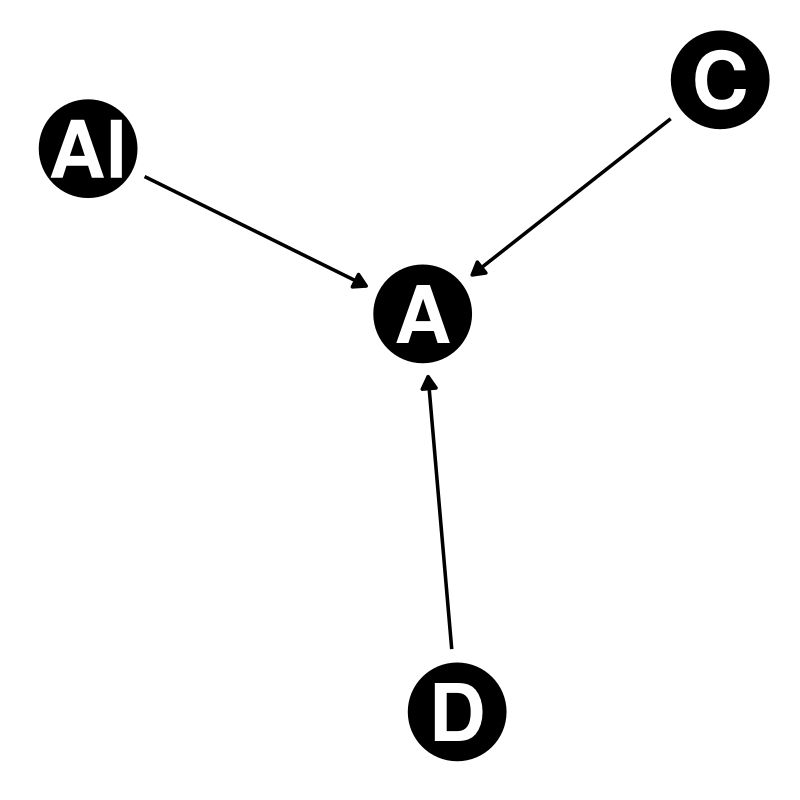
\includegraphics[width=0.40\textwidth]{../fala/plots/dag_non_canonical_agreement.png}
  \end{center}
\end{frame}

\begin{frame}
  \frametitle{Domínio da atração: classe de palavras e infinitivo copular}

  {
    \ex.Hierarquias de Predicados e Concordância~(\cite[233]{Corbett2006}):\\
    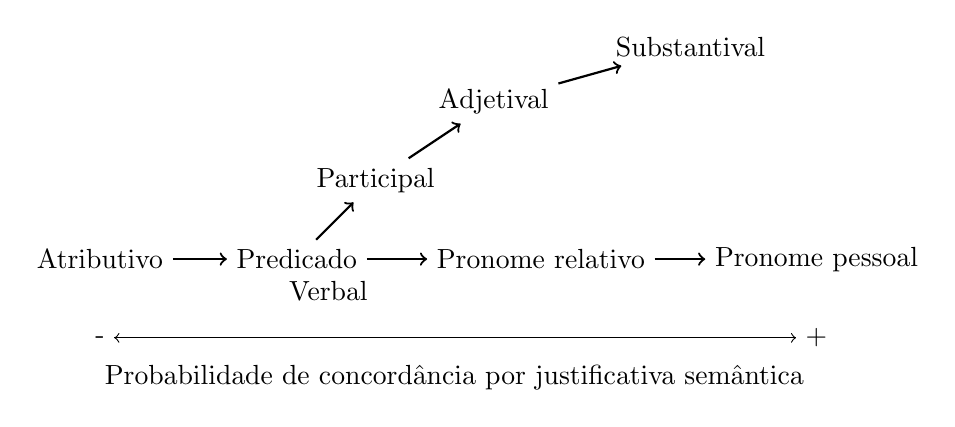
\begin{tikzpicture}[baseline=0pt]
      \node (attr) at (0, 0) {Atributivo};
      \node (pred) at (2.5, 0) {Predicado};
      \node (predv) at (2.9, -0.4) {Verbal};
      \node (predp) at (3.5, 1) {Participal};
      \node (preda) at (5, 2) {Adjetival};
      \node (predn) at (7.5, 2.7) {Substantival};
      \node (relp) at (5.6, 0) {Pronome relativo};
      \node (perp) at (9.1, 0) {Pronome pessoal};
      \node (less) at (0, -1) {-};
      \node (plus) at (9.1, -1) {+};
      \draw[->, thick] (attr) to (pred);
      \draw[->, thick] (pred) to (relp);
      \draw[->, thick] (relp) to (perp);
      \draw[->, thick] (pred) to (predp);
      \draw[->, thick] (predp) to (preda);
      \draw[->, thick] (preda) to (predn);
      \draw[->] (less) to (plus);
      \draw[->] (plus) to (less);
      \node at (4.5, -1.5) {Probabilidade de concordância por justificativa
        semântica};
    \end{tikzpicture}

  }

\end{frame}

\begin{frame}
  \frametitle{Domínio da atração: DAG}
  \begin{center}
    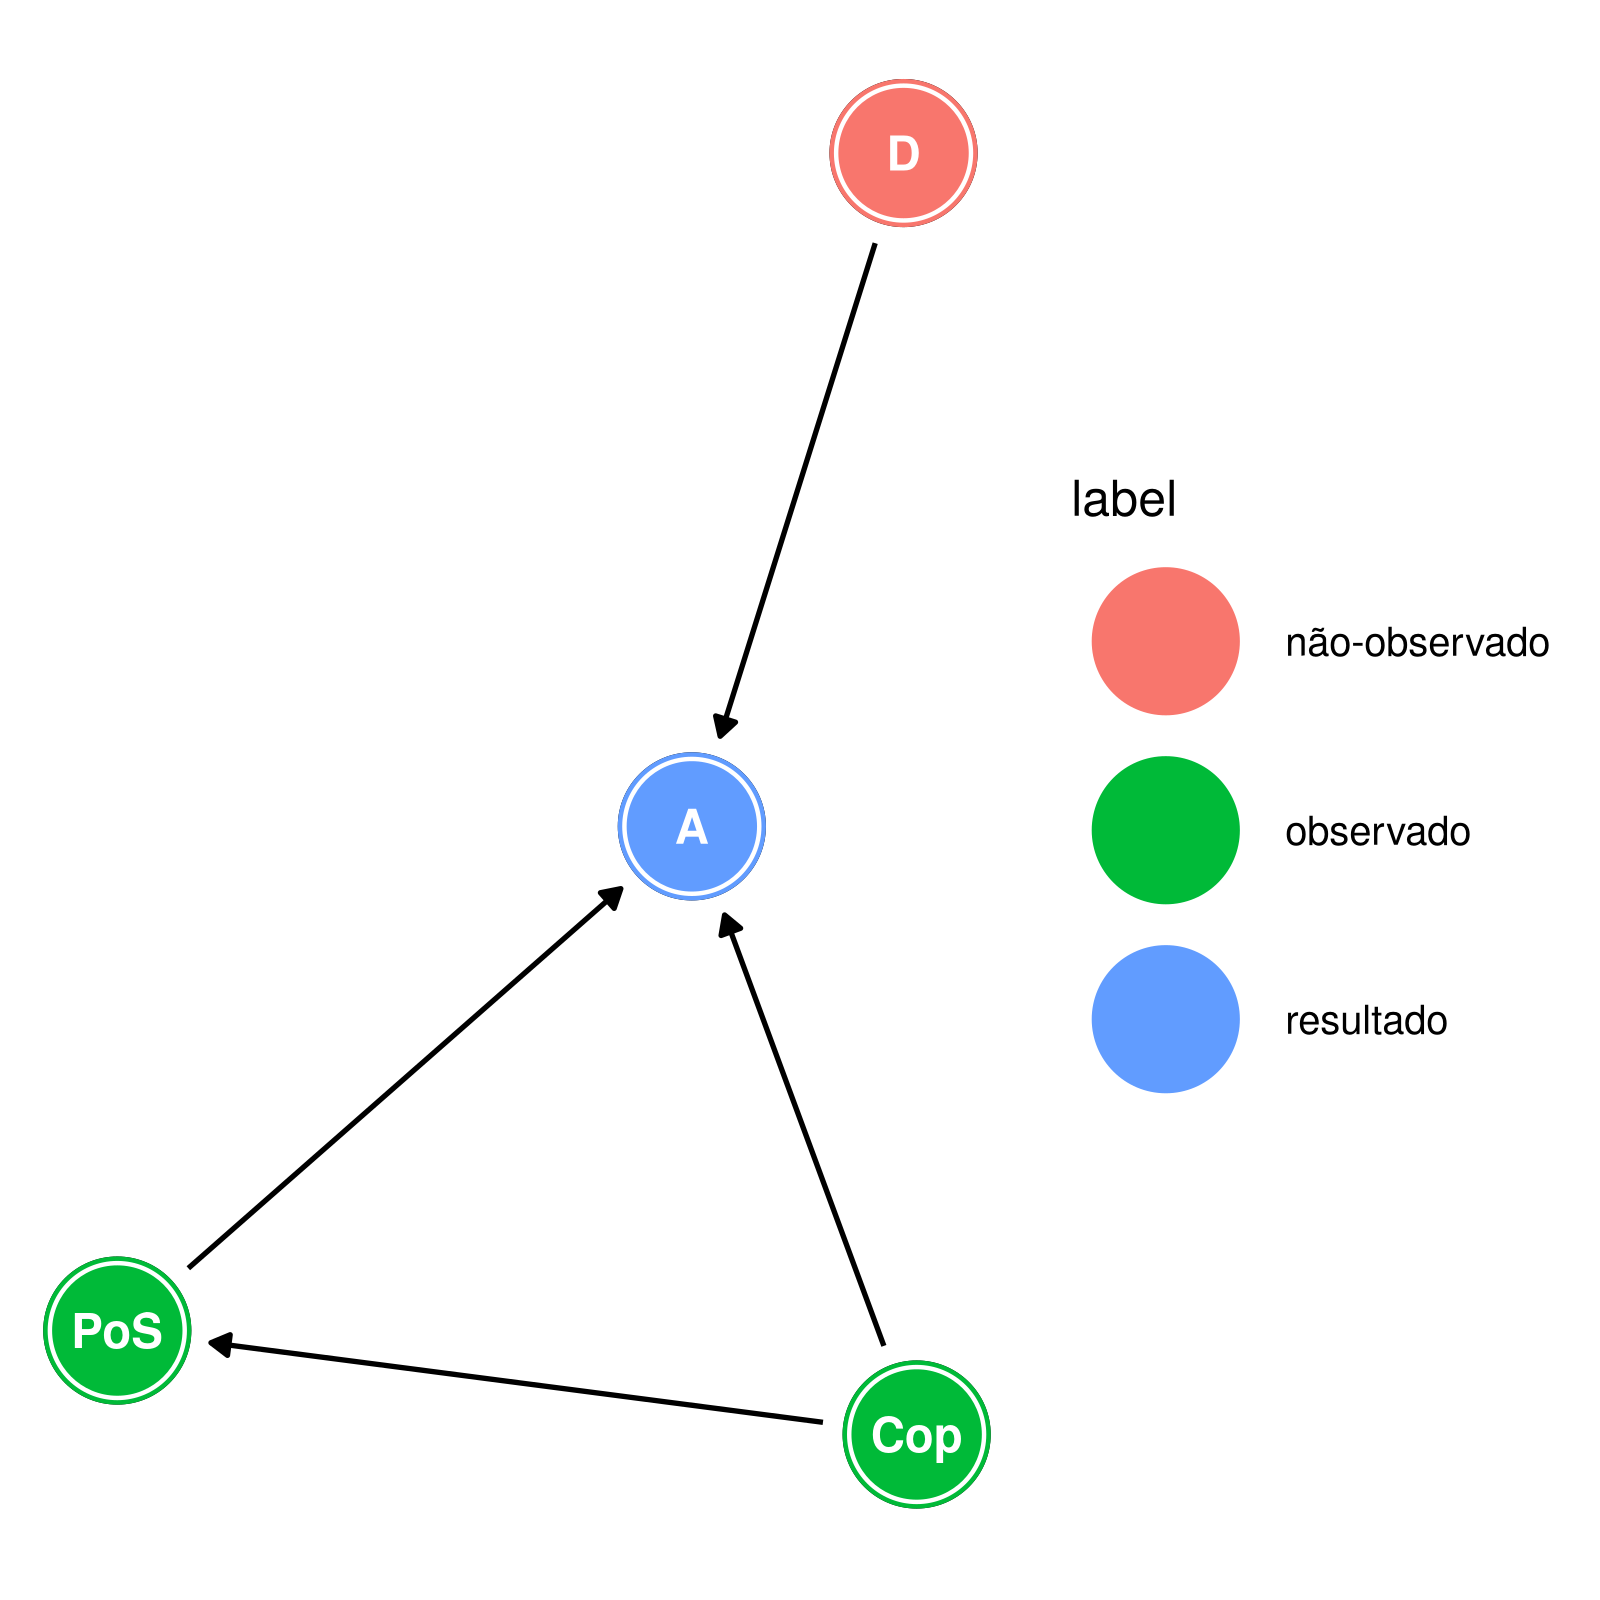
\includegraphics[width=0.65\linewidth]{../fala/plots/dag_a.png}
  \end{center}
\end{frame}

\begin{frame}
  \frametitle{Controlador da atração: papel temático}
  \ex. ἀλλ᾽ ἐξαρκῇ \textbf{σοι} τὰ ἔργα αὐτῶν \textbf{ὁρῶντι} σέβεσθαι καὶ τιμᾶν
  τοὺς θεούς.\\
  Mas é suficiente a ti olhar esses feitos e respeitar e honrar os deuses.
  (Xen.\ \emph{Mem.} 4.3.13)

\end{frame}

\begin{frame}
  \frametitle{Controlador da atração: DAG}
  \begin{center}
    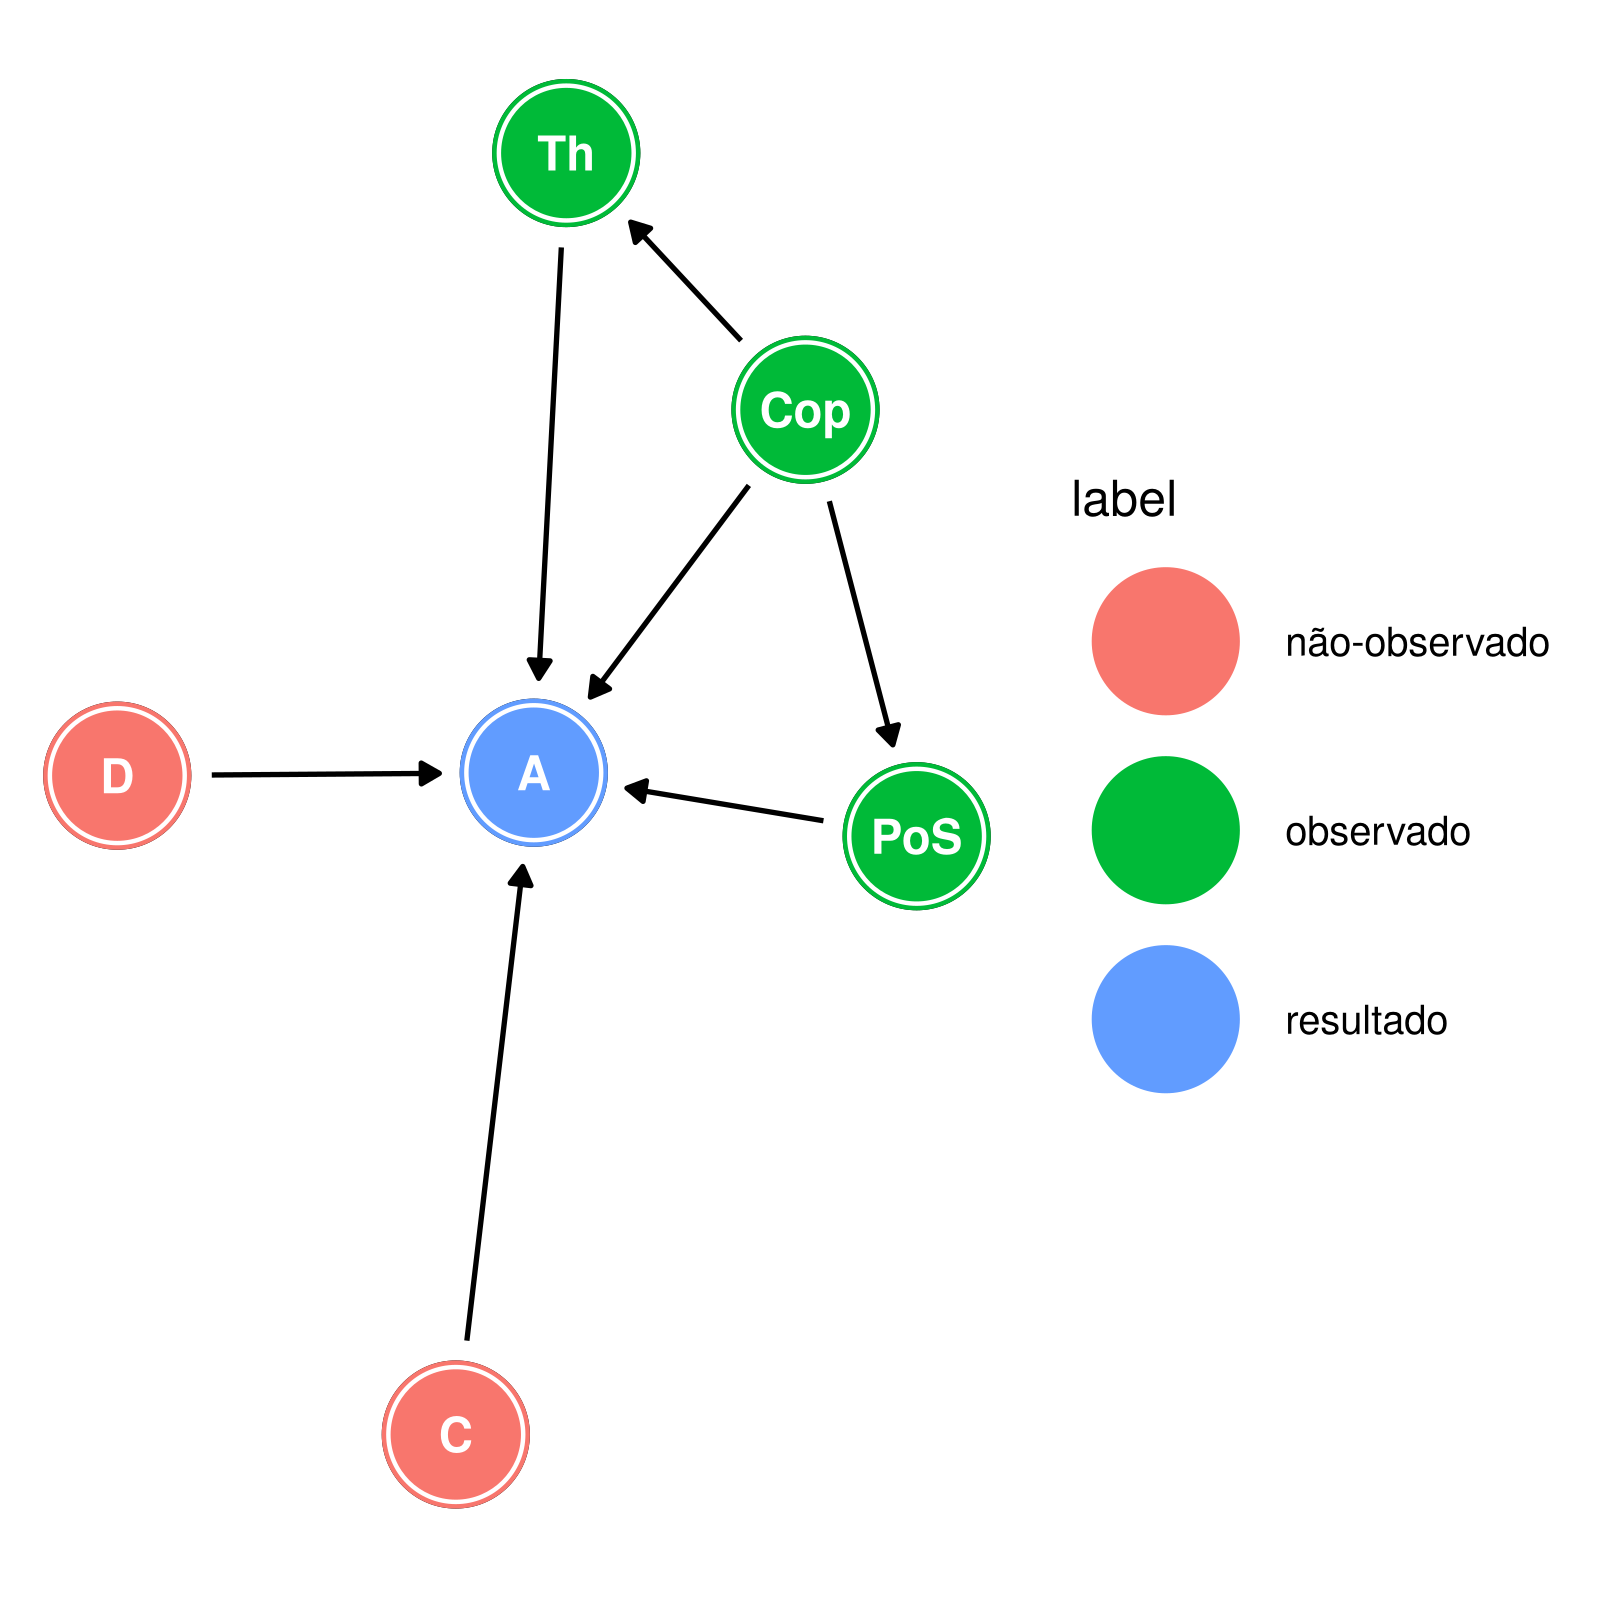
\includegraphics[width=0.65\linewidth]{../fala/plots/dag_b.png}
  \end{center}
\end{frame}

\begin{frame}
  \frametitle{Questões de dialeto e autoria: DAG}
  \begin{center}
    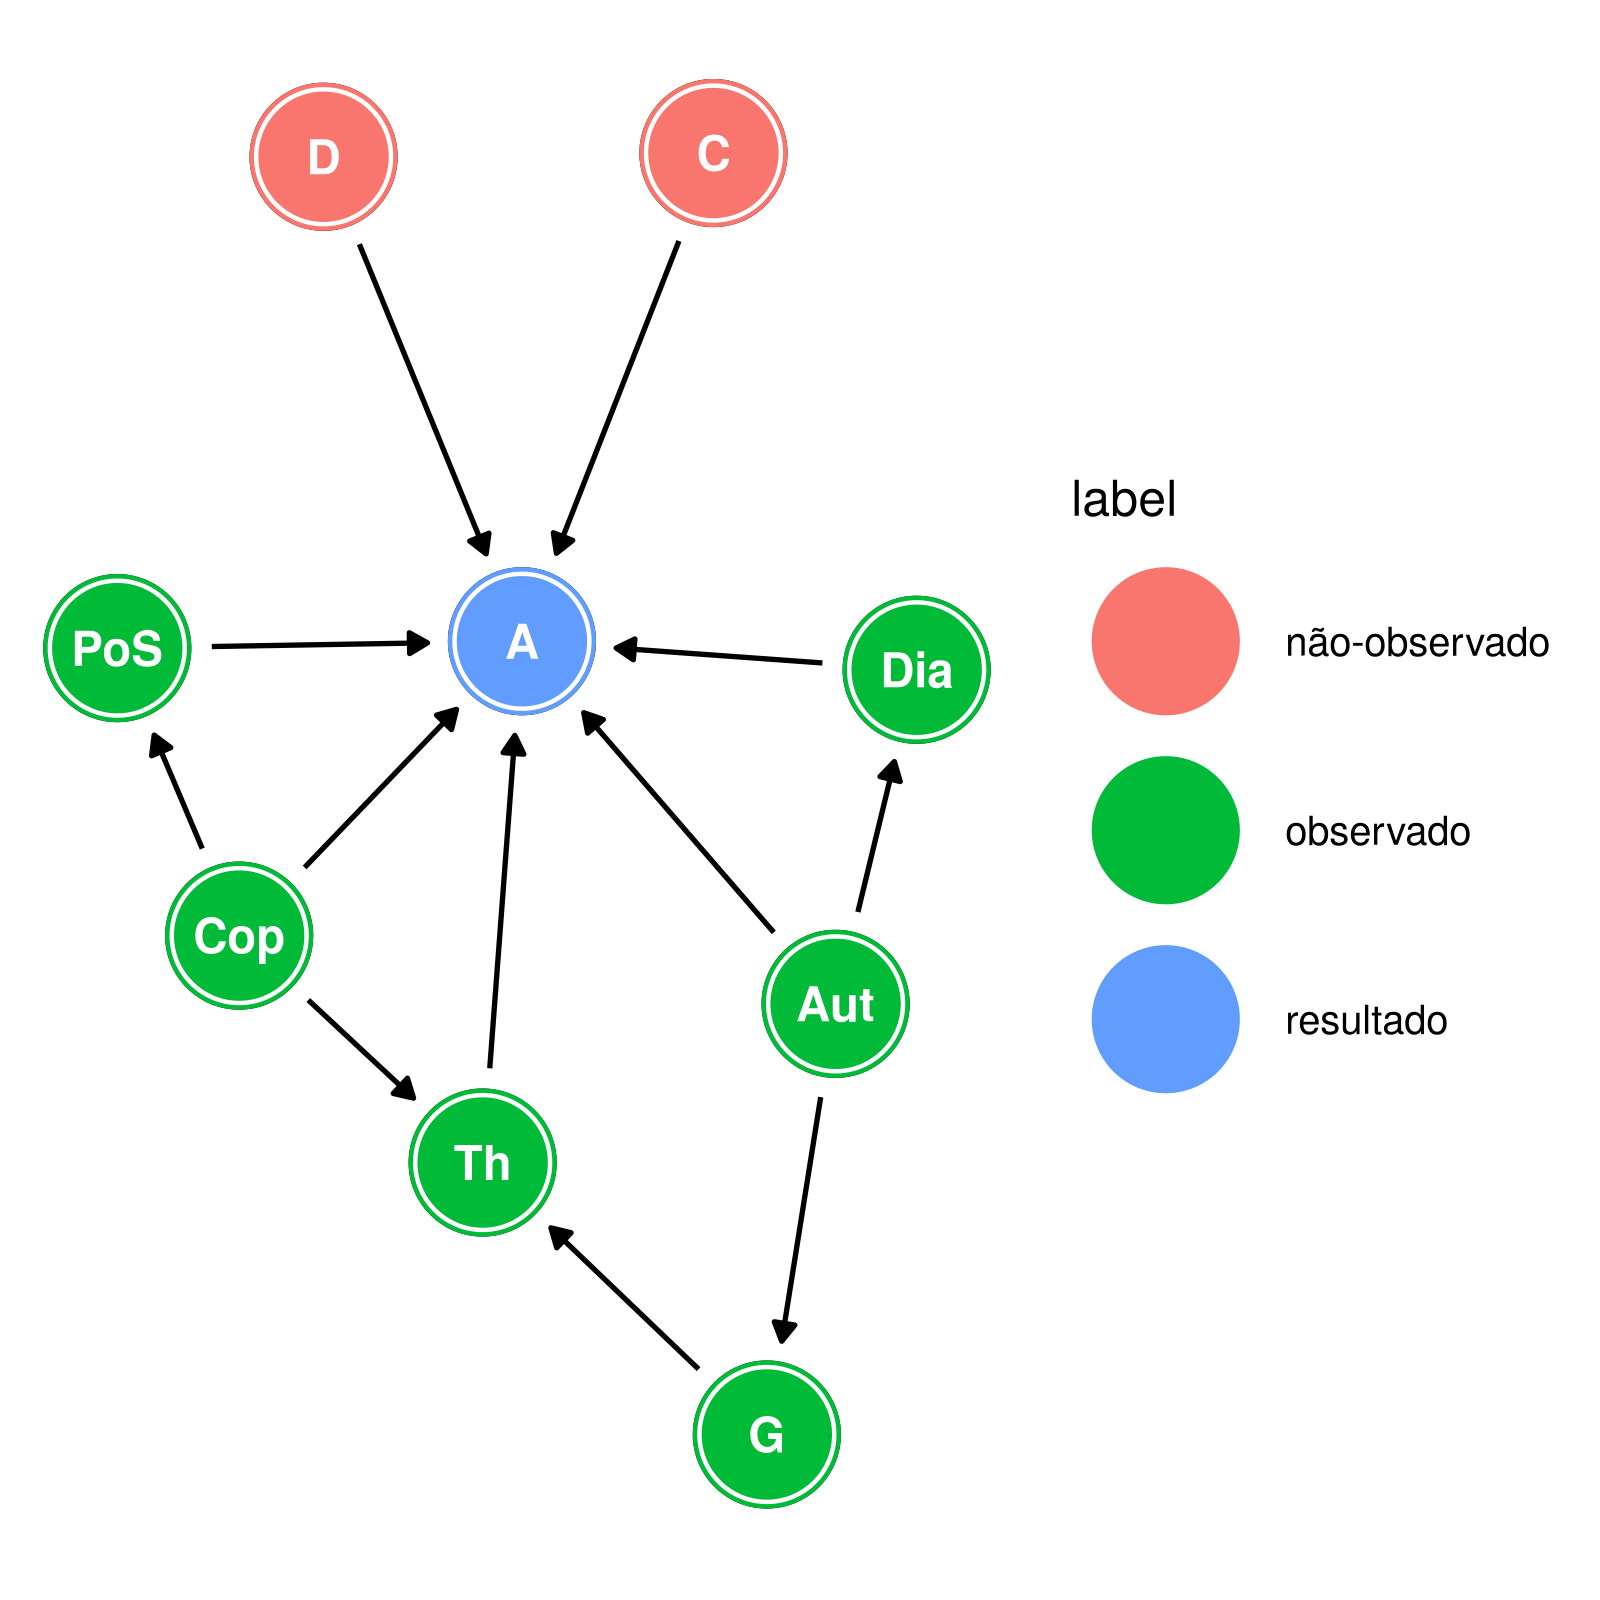
\includegraphics[width=0.65\linewidth]{../fala/plots/dag_c.png}
  \end{center}
\end{frame}

\begin{frame}
  \frametitle{Alvo da atração: distância e precedência}
  \ex.ὡς \textbf{ἀγαθοῖς} τε \textbf{ὑμῖν} προσήκει εἶναι.\\
  Que a vós seja dado ser boa gente. (Xen.\ \emph{Anab.} 3.2.11)

\end{frame}

\begin{frame}
  \frametitle{Alvo da atração: DAG final}

  \begin{center}
    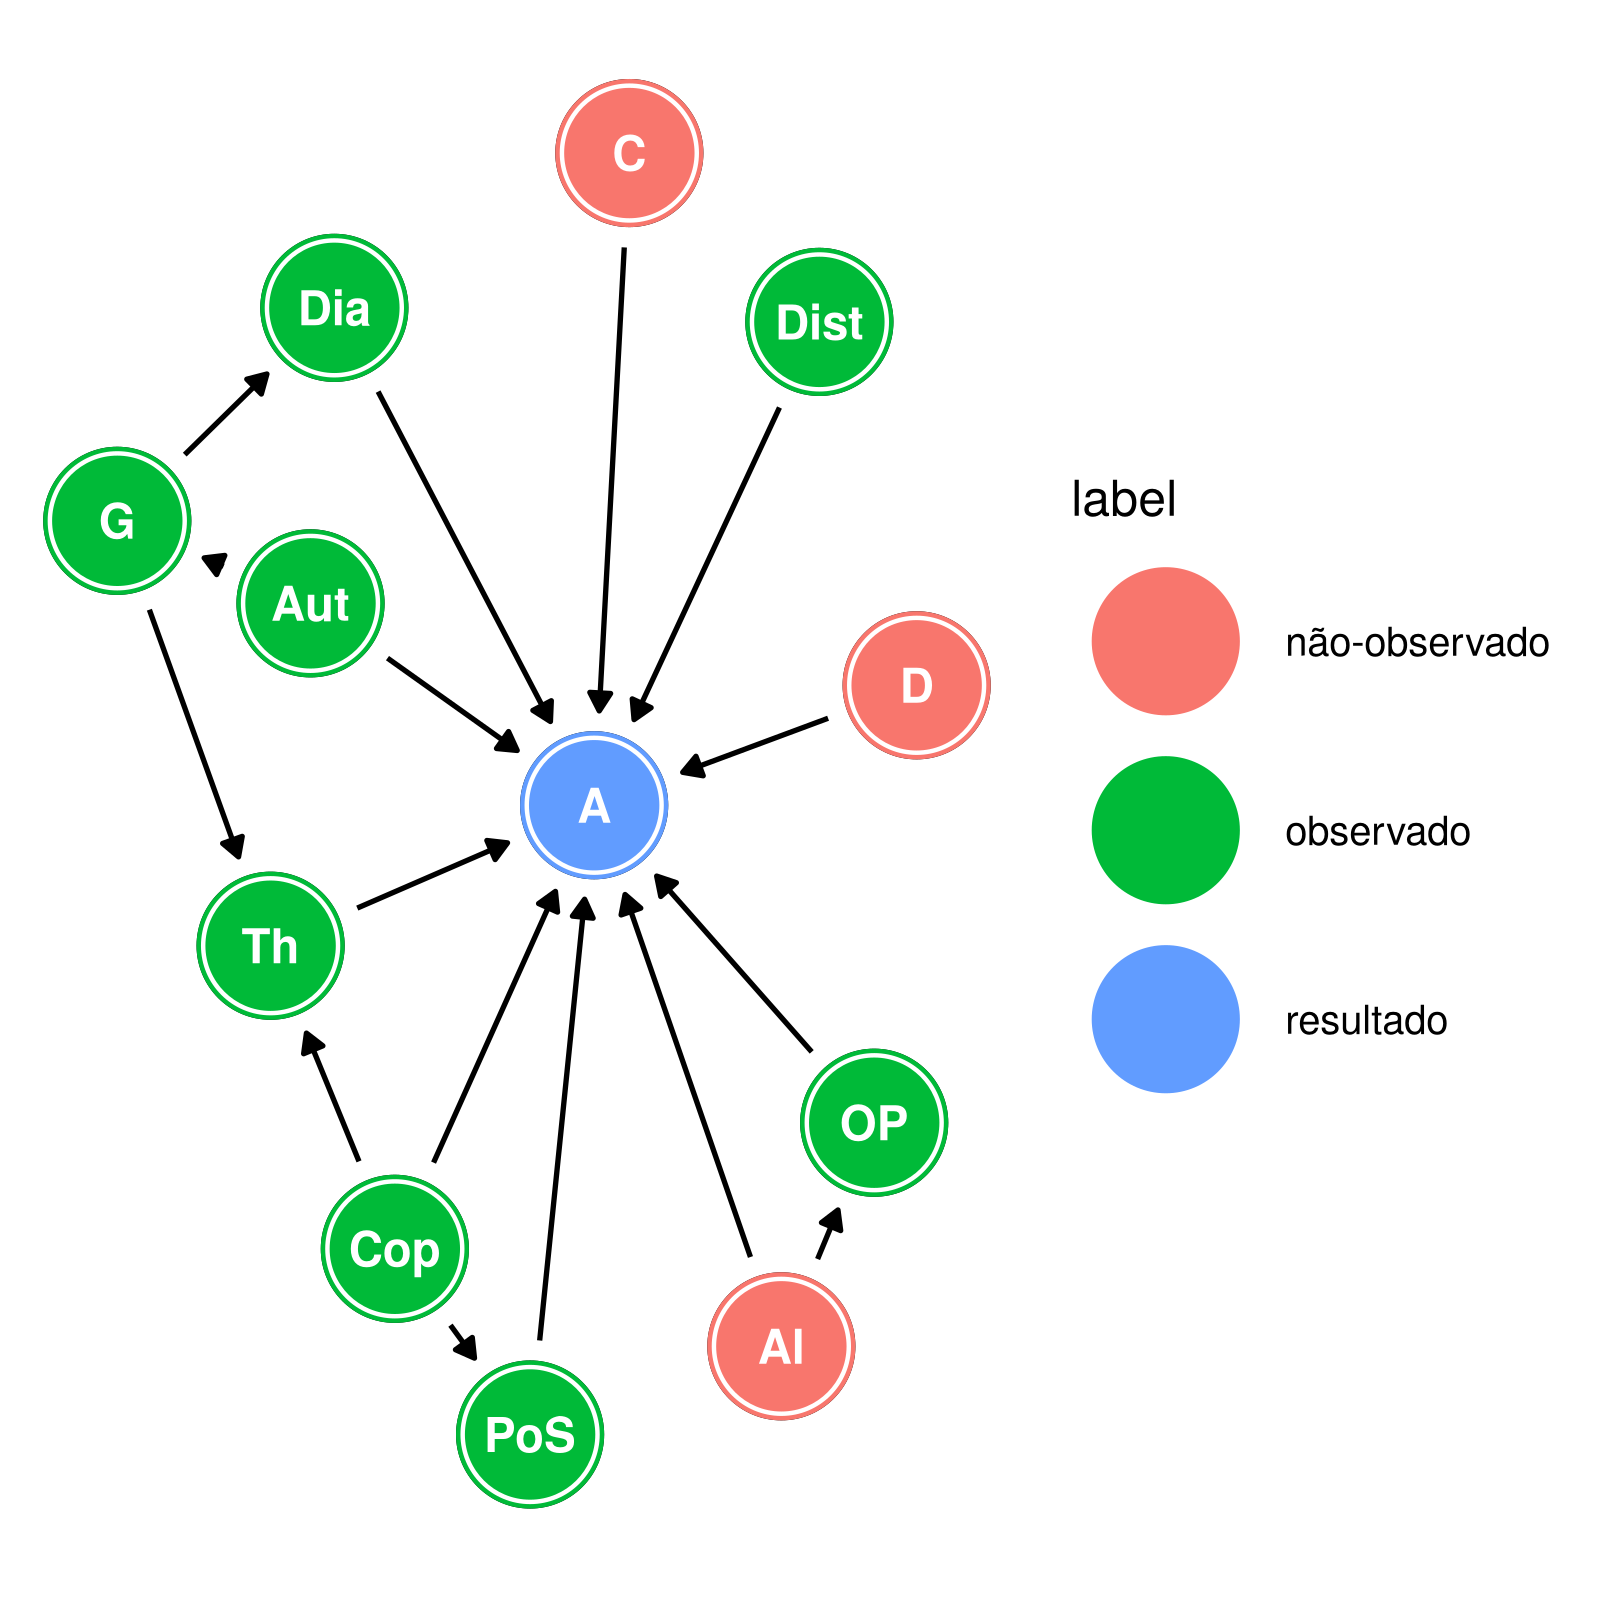
\includegraphics[width=0.60\linewidth]{../fala/plots/dag_d.png}
  \end{center}

  \vfill


  \footnotesize

  \textbf{Ferramentas:} R (\cite{R}), pacotes
  \texttt{tidyverse} (\cite{tidyverse}), \texttt{dagitty} (\cite{dagitty}),
  \texttt{ggdag} (\cite{ggdag}) e \texttt{rethinking} (\cite{McElreath2020}),
  bem como o software Stan~(\cite{StanReferenceManual,StanUserGuide}).

\end{frame}

\begin{frame}
  \frametitle{Modelo Linear Generalizado}
  \small
  \begin{align*}
    \text{A}                                                & \sim \Bernoulli(p_i)                                     \\
    \logit(p_i)                                             & = \alpha_{\Sent} + \bv{Cop}\Cop_i + \bv{Dist}|\Dist_i| + \\
                                                            & +
    \bv{PoS}\sum^{\PoS_{i}-1}_{j=0}{\delta_{j_{\PoS}}} +\bv{Th}\sum^{Th_{i}-1}_{j=0}{\delta_{j_{\Th}}}                 \\
                                                            & + \bvi{Auth} + \bvi{Dia}                                 \\
    \alpha                                                  & = \abar_\Sent + z_{\Sent} * \sigma_\Sent                 \\
    \bv{Cop}, \bv{Dist}                                     & \sim \Normal(0, 1)                                       \\
    \bv{PoS}, \bv{Th}                                       & \sim \Normal(0, 1)                                       \\
    \delta_{\PoS}, \delta_{\Th}                             & \sim \Dirichlet(2)                                       \\
    \bv{Auth}                                               & = z_{\Auth}*\sigma_{\Auth}                               \\
    \bv{Dia}                                                & = \bbar_\Dia + z_{\Dia}*\sigma_{\Dia}                    \\
    \abar_\Sent, \bbar_\Dia, z_{\Sent}, z_{\Auth}, z_{\Dia} & \sim \Normal(0,1)                                        \\
    \sigma_{\Sent}, \sigma_{\Auth}, \sigma_{\Dia}           & \sim \Exponencial(1)
  \end{align*}
\end{frame}

\begin{frame}
  \frametitle{Sobre Preditores Categóricos Ordenados}

  \begin{center}
    \begin{tabular}[t]{ll}
      \toprule
      PoS        & Cummulative effect                                                  \\
      \midrule
      Participle & $\beta_{\text{PoS}} * 0$                                            \\
      Adjective  & $\beta_{\text{PoS}} * (\delta_{\text{Adj}})$                        \\
      Noun       & $\beta_{\text{PoS}} * (\delta_{\text{Adj}} + \delta_{\text{Noun}})$ \\
      \bottomrule
    \end{tabular}
  \end{center}

\end{frame}

\begin{frame}
  \frametitle{Cópula e distância}
  \begin{center}
    
\begin{tabular}[t]{lrrrrr}
\toprule
Effect & mean & sd & 5.5\% & 94.5\% & rhat\\
\midrule
$\beta_{\text{Copula}}$ & 1.81 & 0.47 & 1.07 & 2.57 & 1.00\\
$\beta_{\text{Dist}}$ & -0.27 & 0.06 & -0.37 & -0.18 & 1.01\\
\bottomrule
\end{tabular}

    \begin{figure}[!h]
      \centering
      \begin{minipage}{.40\textwidth}
        \centering
        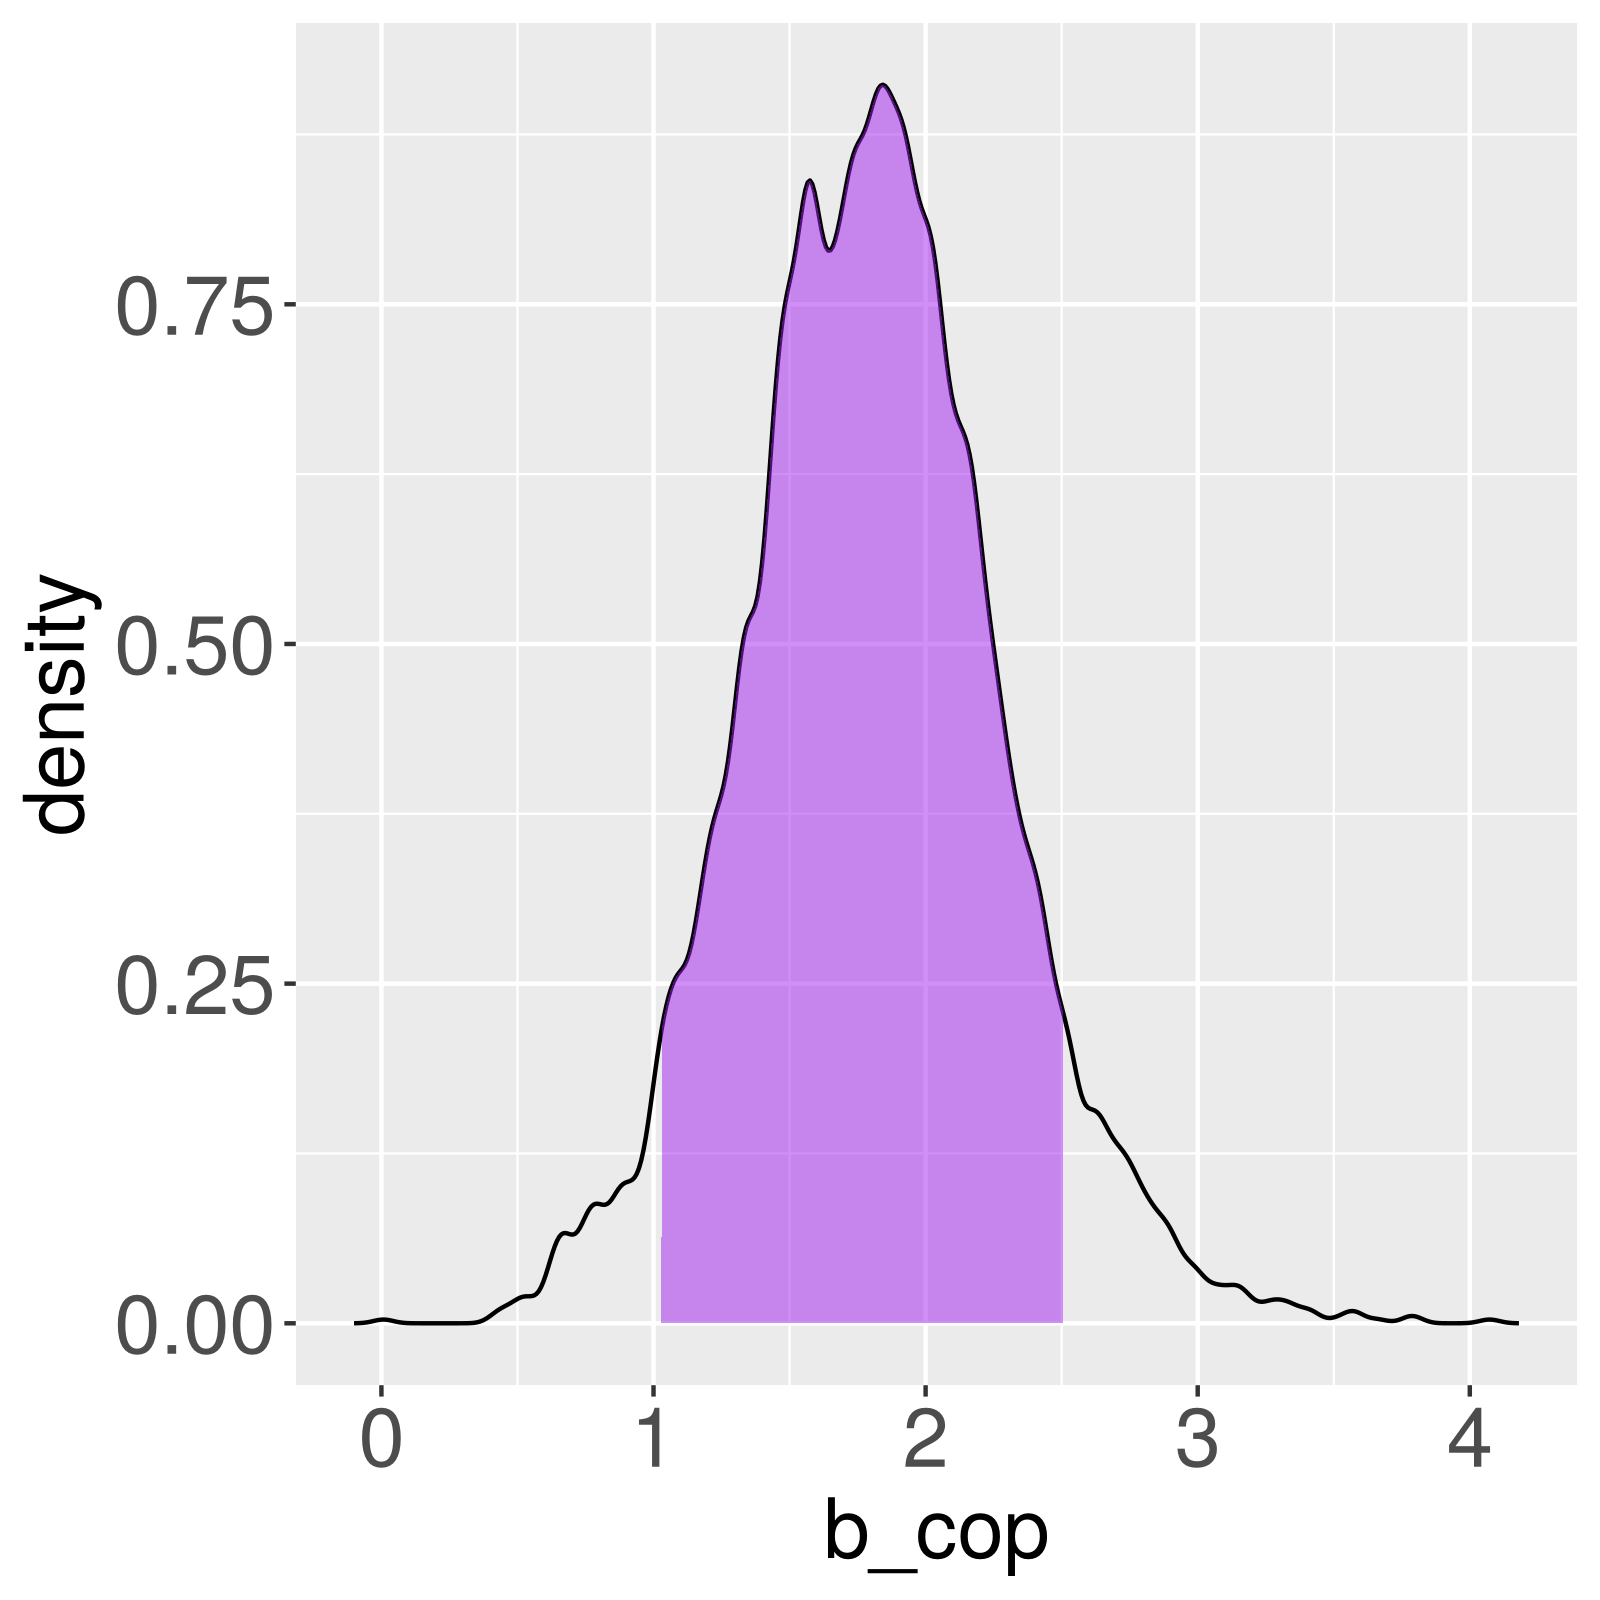
\includegraphics[width=\linewidth]{../fala/plots/posterior_b_copula.png}
      \end{minipage}%
      \hspace{3em}
      \begin{minipage}{.40\textwidth}
        \centering
        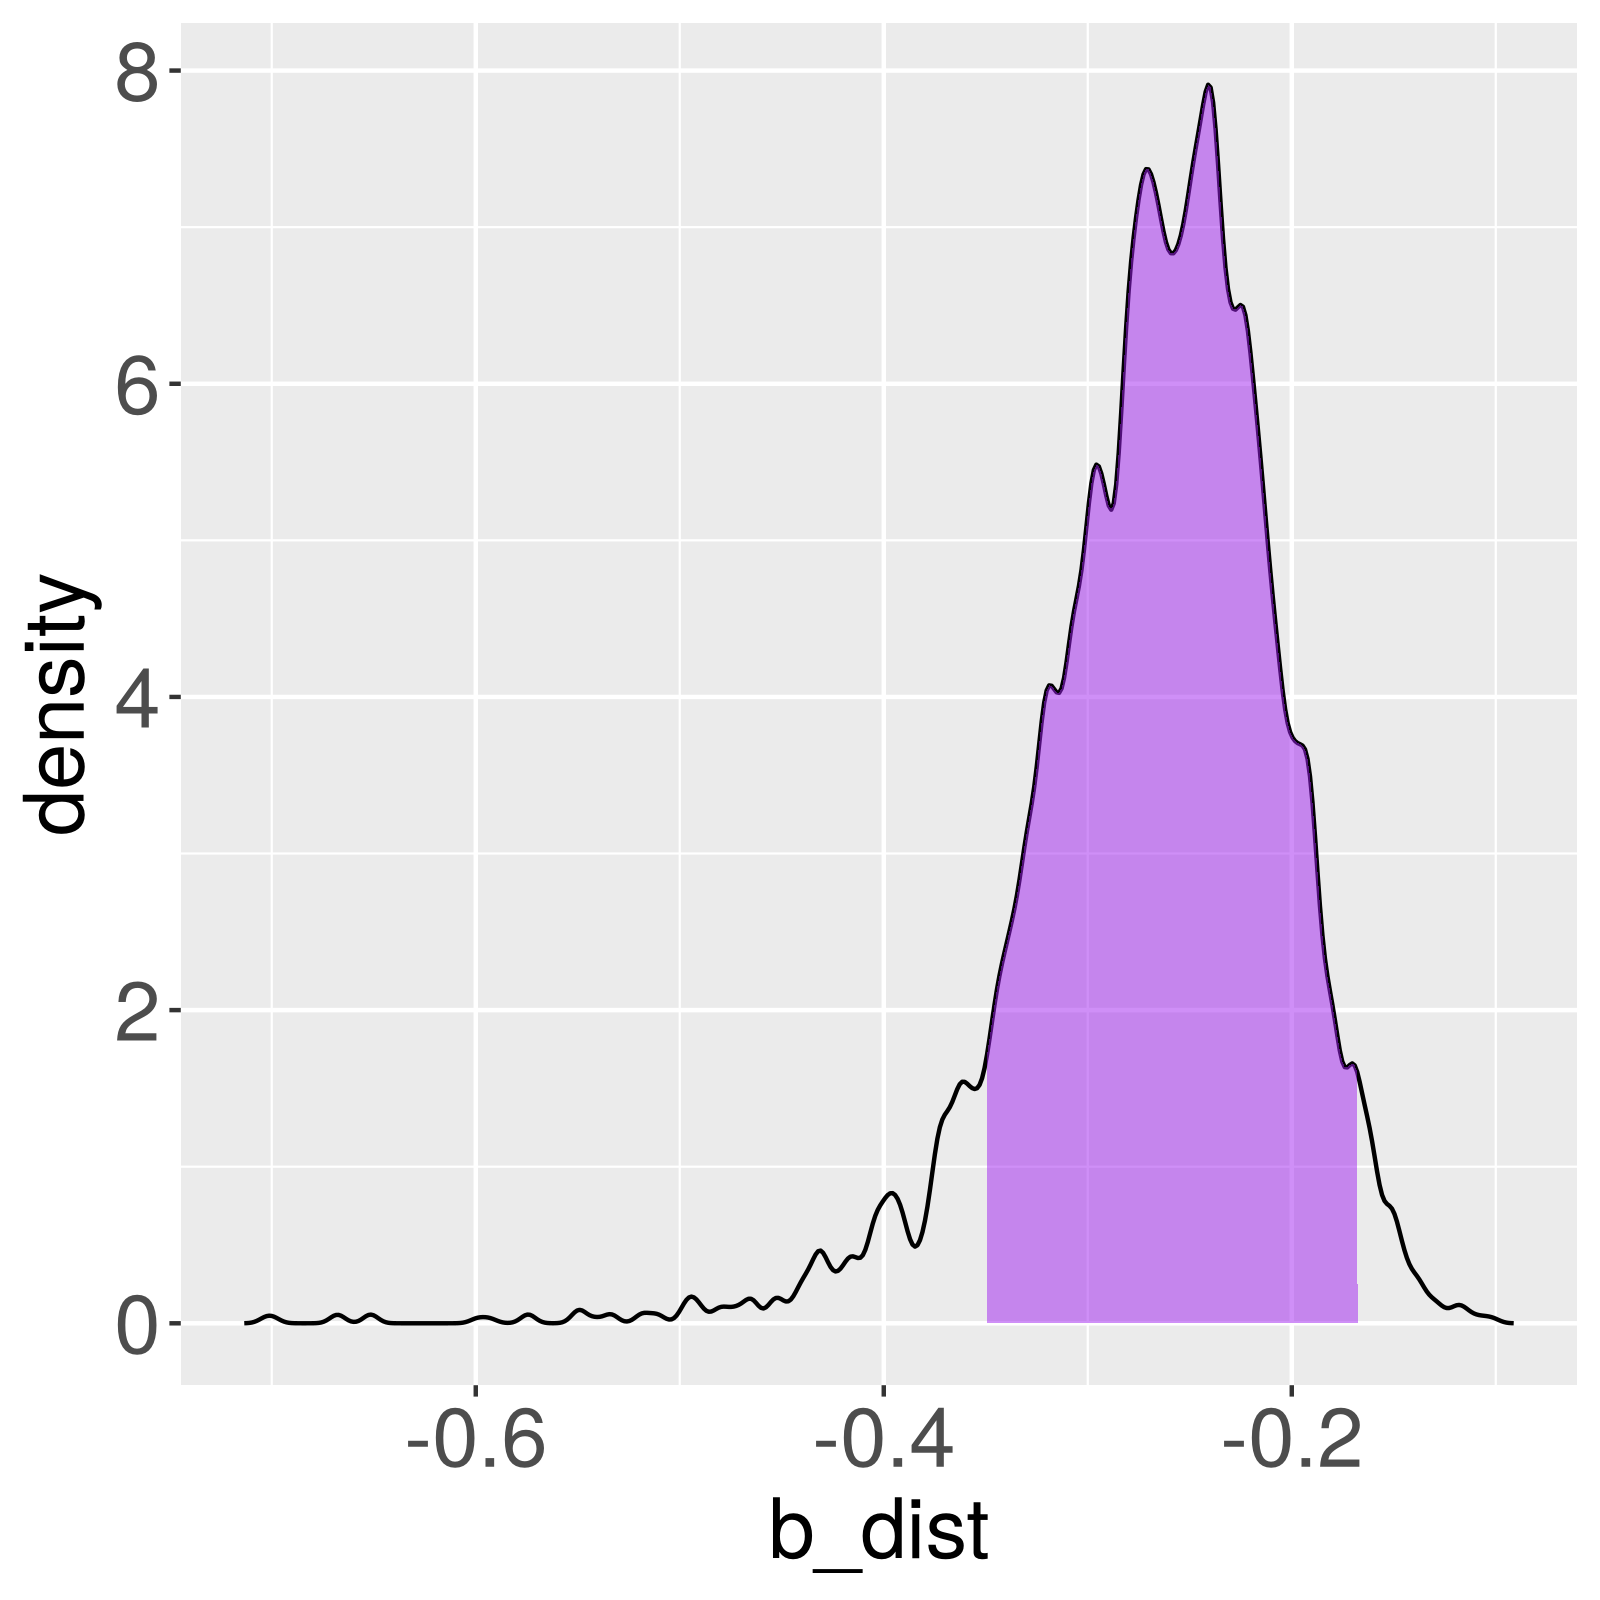
\includegraphics[width=\linewidth]{../fala/plots/posterior_b_dist.png}
      \end{minipage}
    \end{figure}
  \end{center}

\end{frame}

\begin{frame}
  \frametitle{Classe de palavras e hierarquia de predicados}
  \small
  \begin{center}
    
\begin{tabular}[t]{lrrrrr}
\toprule
Effect & mean & sd & 5.5\% & 94.5\% & rhat\\
\midrule
$\beta_{\text{PoS}}$ & 0.76 & 0.51 & 0.17 & 1.71 & 1\\
$\delta_{\text{Adj}}$ & 0.48 & 0.18 & 0.19 & 0.78 & 1\\
$\delta_{\text{Noun}}$ & 0.52 & 0.18 & 0.22 & 0.81 & 1\\
\bottomrule
\end{tabular}

    
\begin{tabular}[t]{llrrrrr}
\toprule
PoS & Cummulative effect & mean & sd & 5.5\% & 94.5\% & rhat\\
\midrule
Participle & $\beta_{\text{PoS}} * 0$ & 0.00 & 0.00 & 0.00 & 0.00 & --\\
Adjective & $\beta_{\text{PoS}} * \delta_{\text{Adj}}$ & 0.35 & 0.26 & 0.06 & 0.86 & 1\\
Noun & $\beta_{\text{PoS}} * (\delta_{\text{Adj}} + \delta_{\text{Noun}})$ & 0.76 & 0.51 & 0.17 & 1.71 & 1\\
\bottomrule
\end{tabular}

  \end{center}
\end{frame}

\begin{frame}
  \frametitle{Papel temático do controlador}
  \small
  \begin{center}
    
\begin{tabular}[t]{lrrrrr}
\toprule
Effect & mean & sd & 5.5\% & 94.5\% & rhat\\
\midrule
$\beta_{\text{Theta}}$ & 2.73 & 0.60 & 1.88 & 3.76 & 1\\
$\delta_{\text{Exp}}$ & 0.38 & 0.12 & 0.19 & 0.57 & 1\\
$\delta_{\text{Agent}}$ & 0.62 & 0.12 & 0.43 & 0.81 & 1\\
\bottomrule
\end{tabular}

    \bigskip
    
\begin{tabular}[t]{llrrrrr}
\toprule
Theta & Cummulative effect & mean & sd & 5.5\% & 94.5\% & rhat\\
\midrule
Recipient & $\beta_{\text{Th}} * 0$ & 0.00 & 0.00 & 0.00 & 0.00 & --\\
Experiencer & $\beta_{\text{Th}} * \delta_{\text{Exp}}$ & 1.04 & 0.41 & 0.44 & 1.73 & 1\\
Agent & $\beta_{\text{Th}} * (\delta_{\text{Exp}} + \delta_{\text{Agent}})$ & 2.73 & 0.60 & 1.88 & 3.76 & 1\\
\bottomrule
\end{tabular}

  \end{center}
\end{frame}

\begin{frame}
  \frametitle{Dialeto}
  \begin{center}
    \small
    
\begin{tabular}[t]{lrrrrr}
\toprule
Effect & mean & sd & 5.5\% & 94.5\% & rhat\\
\midrule
$\overline{\beta}_{\text{Dia}}$ & -0.37 & 0.80 & -1.64 & 0.93 & 1\\
$\sigma_{\text{Dia}}$ & 1.33 & 0.86 & 0.27 & 2.90 & 1\\
$\beta_{\text{Attic}}$ & 0.13 & 0.87 & -1.26 & 1.50 & 1\\
$\beta_{\text{Jonic}}$ & -1.60 & 1.14 & -3.50 & 0.17 & 1\\
$\beta_{\text{Attic}} - \beta_{\text{Jonic}}$ & 1.73 & 0.94 & -0.04 & 3.01 & --\\
\bottomrule
\end{tabular}

    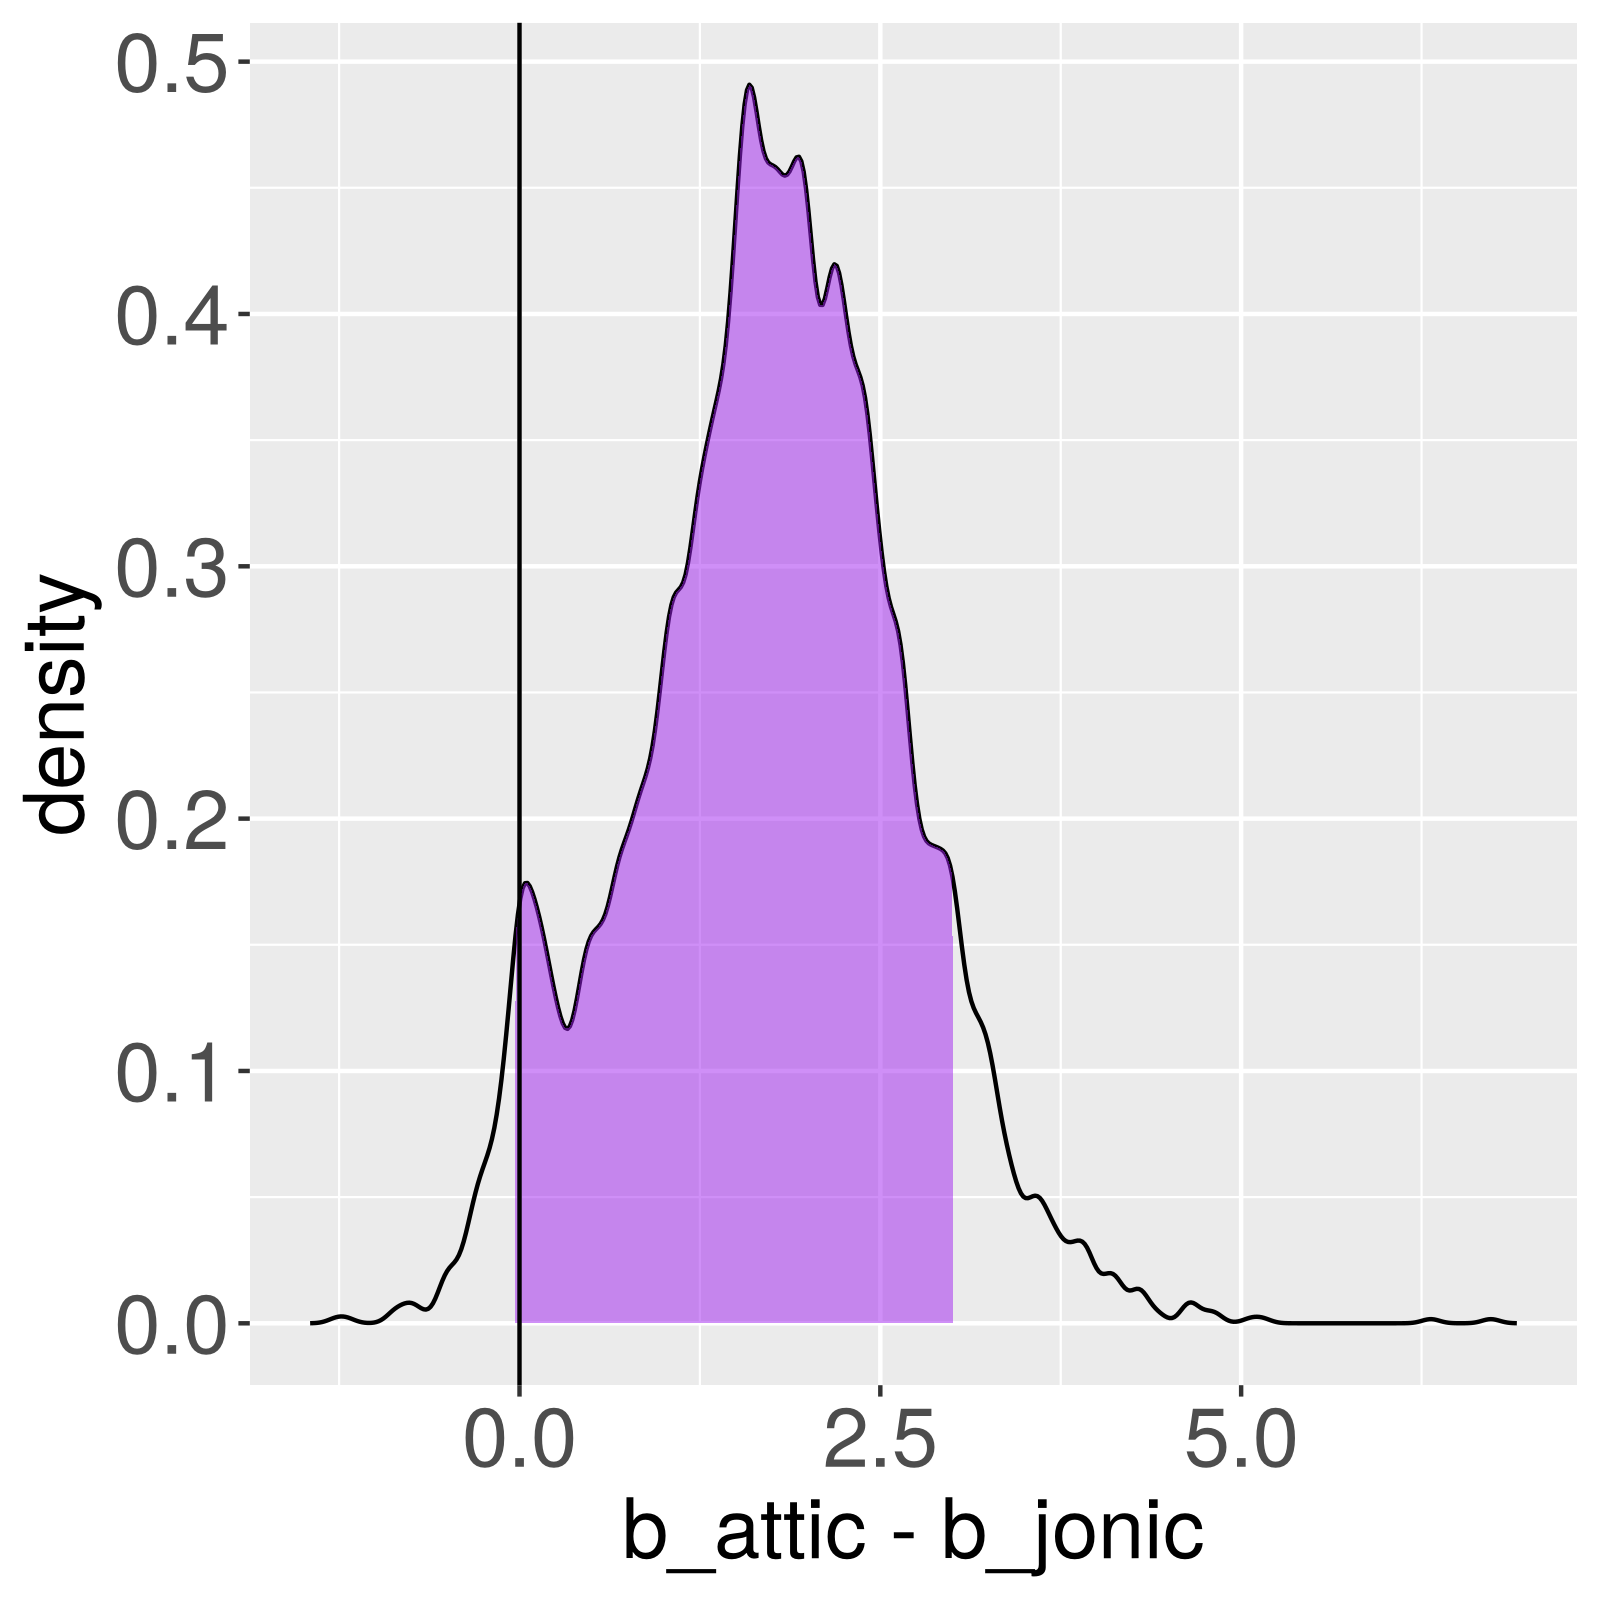
\includegraphics[width=0.4\linewidth]{../fala/plots/posterior_diff_dia.png}
  \end{center}
\end{frame}

\begin{frame}
  \frametitle{Autoria}
  \begin{center}
    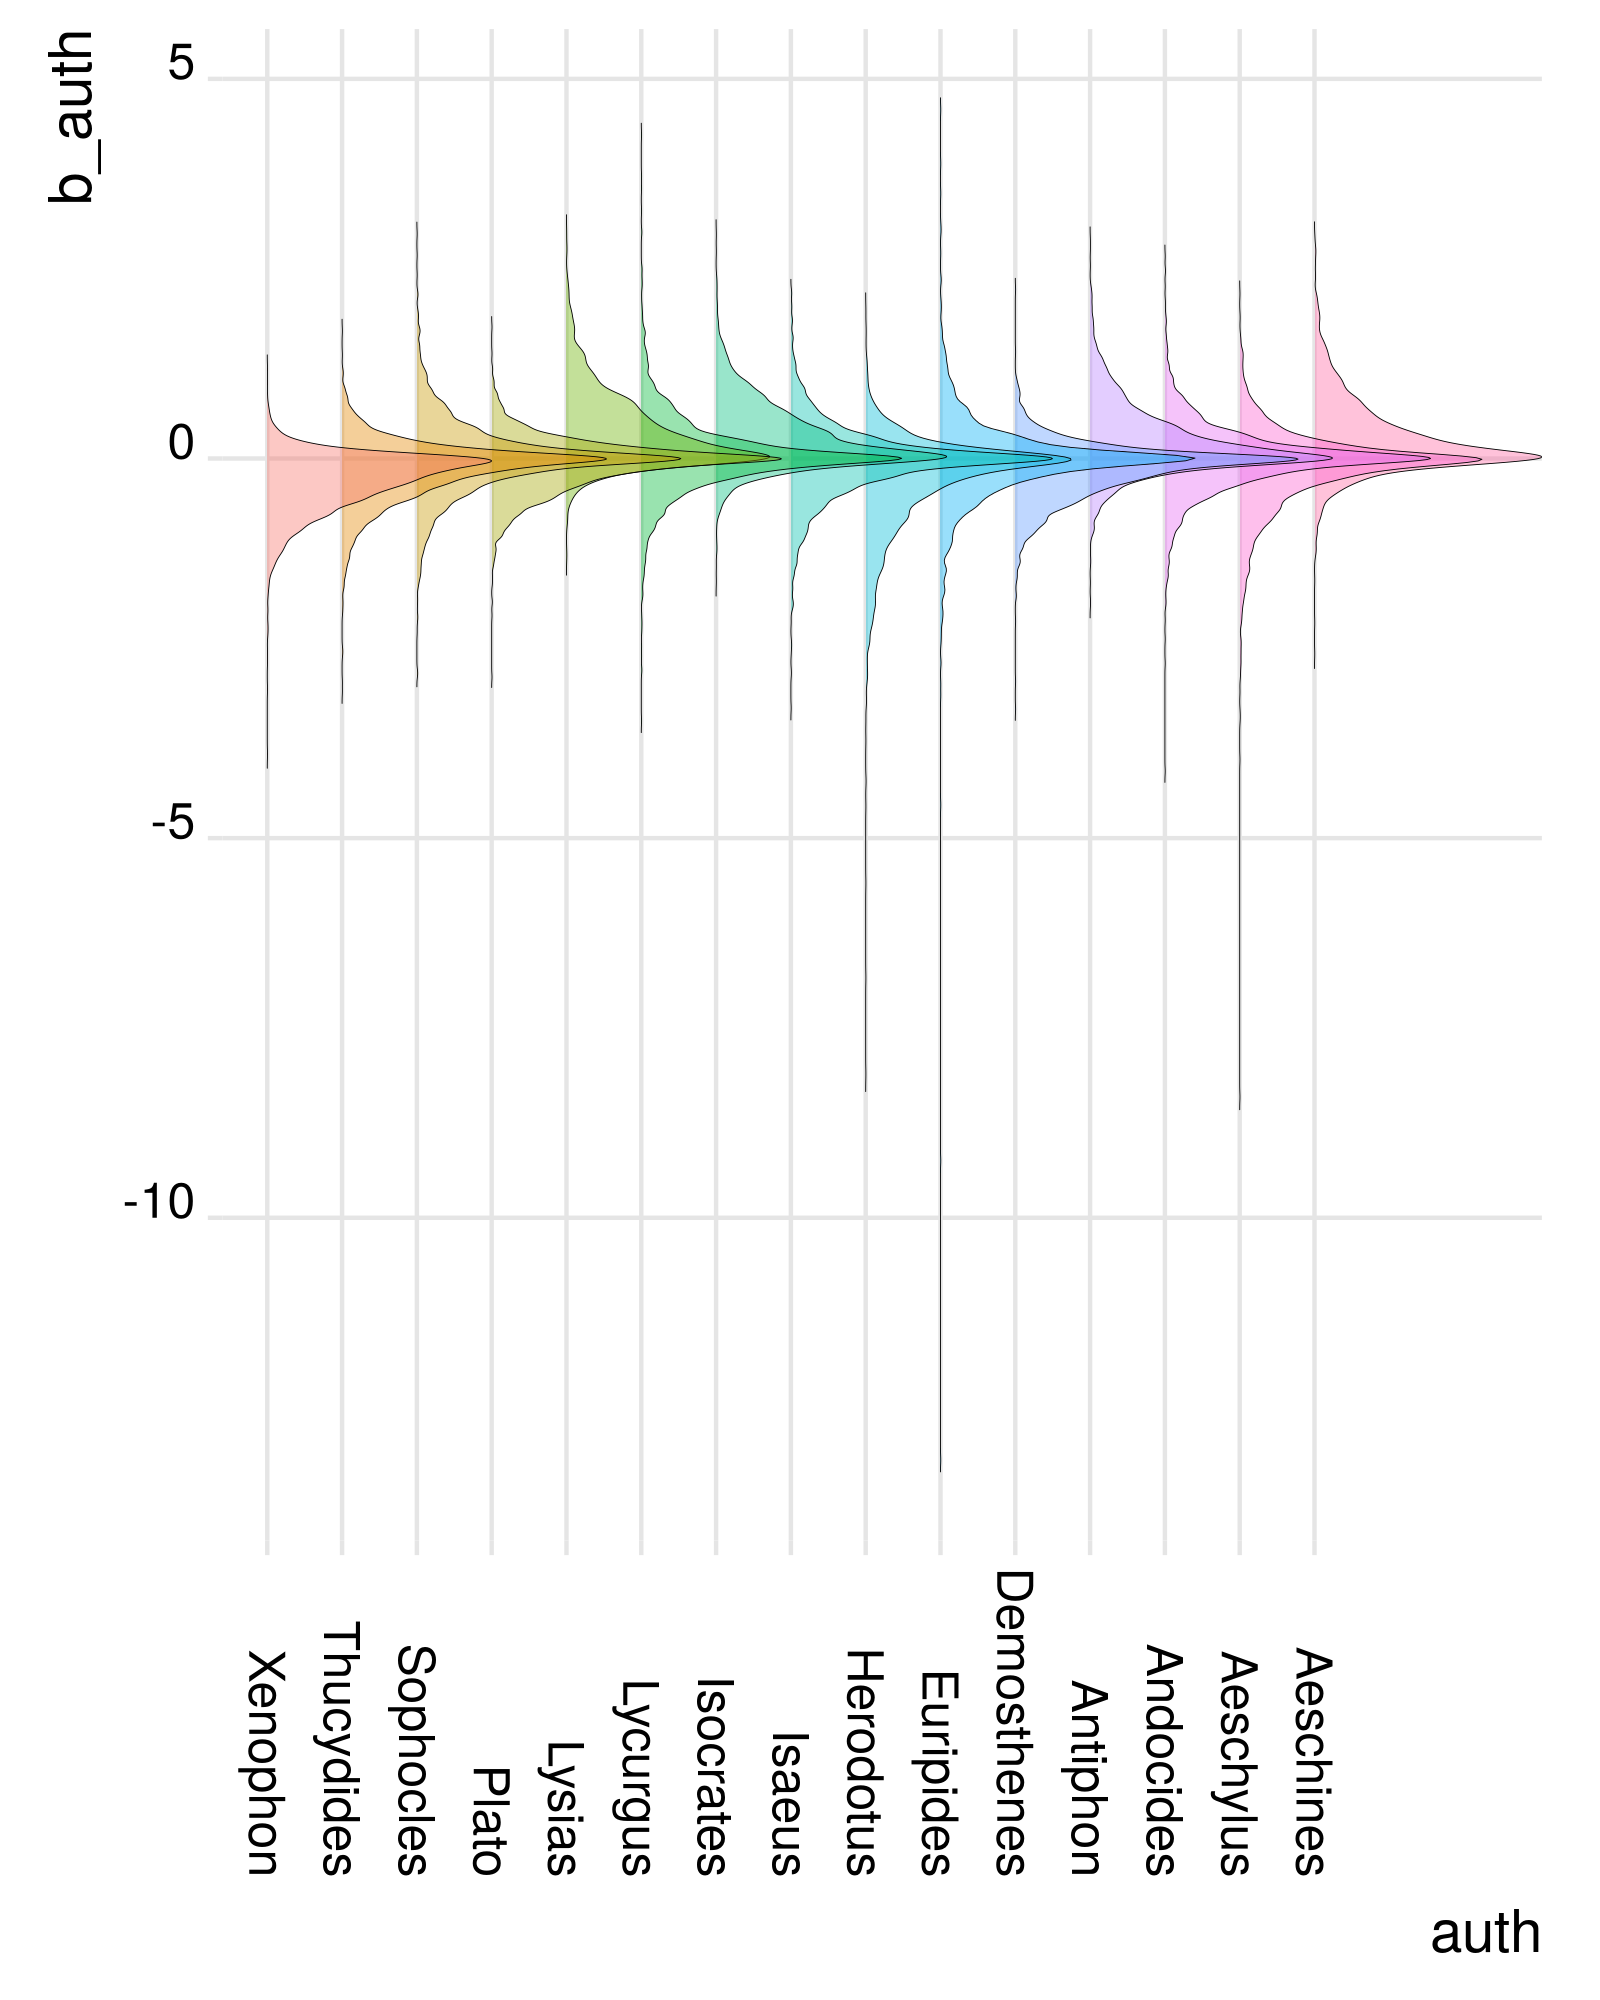
\includegraphics[width=0.70\linewidth,angle=90]{../fala/plots/rainbow_author.png}
  \end{center}
\end{frame}

\begin{frame}
  \begin{center}
    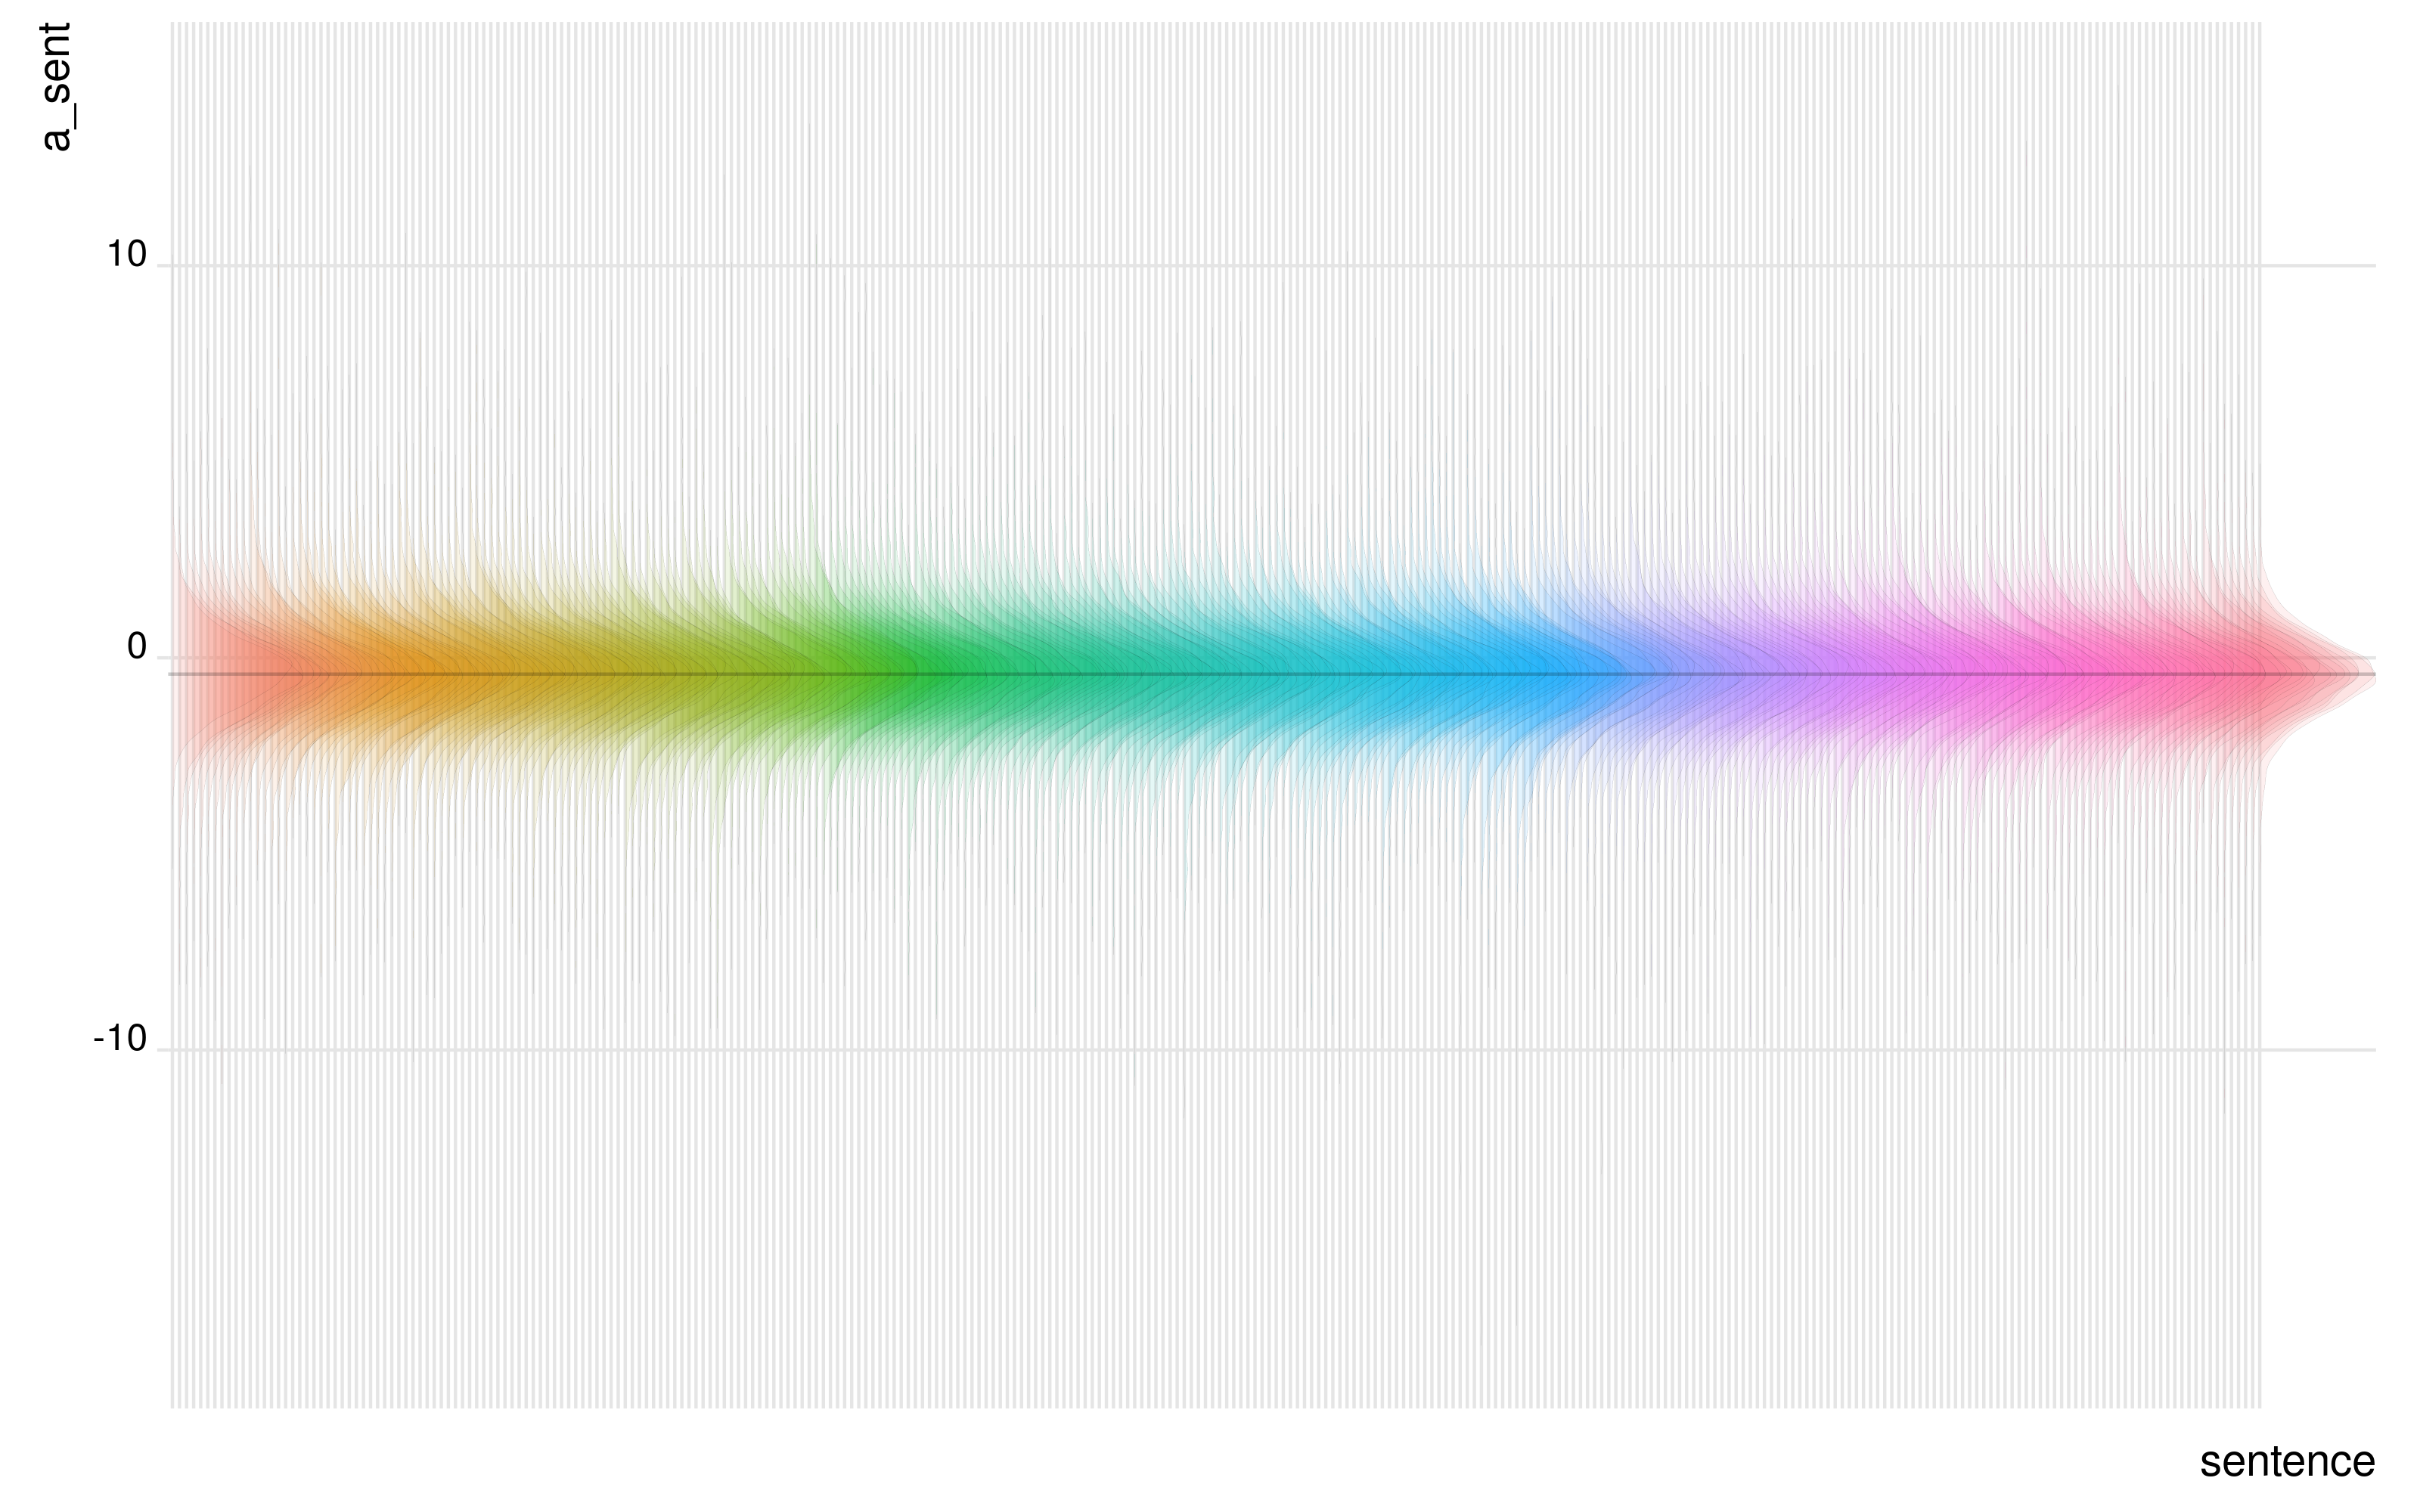
\includegraphics[height=0.75\pageheight]{../fala/plots/rainbow_sent.png}
  \end{center}
\end{frame}

\begin{frame}[standout]
  \large
  Obrigado!
  \bigskip

  Contato:\\
  \texttt{caio.geraldes@usp.com}

  Dados e código disponíveis em\\
  \texttt{github.com/caiogeraldes/sbec2025}
\end{frame}


\end{document}
